\section{Security frameworks}

\subsection{Overview}

When we are talking about the infrastructure security of Kuberntes environment inside the cloud, we must consider multiple layers. Going from the top to the bottom, we start with the security measurements taken on the cloud provider side. In most cases this is not something we can affect and the security of different cloud providers varies significantly. However, all of the ``big five'' cloud providers (AWS, Azure, Google Cloud, Alibaba and IBM) maintain high security standarts and security risks generally should not be a concern for their end users. Then, we get to the cluster itself. On the cluster level we must consider the security of the nodes, security of the cluster components and their configuration. At this layer we have already some space for the misconfigurations to appear. Here we can evaluate the security of the single components using some of the security scanners presented in \nameref{sec:kubernetes-security-automation}. But it should be noted that the cluster can only be as secured as its nodes. Therefore, attention should be given to the node security first. Host operating system should be regularly patched with the most recent security patches. Lastly, we get to the application level, where the security of the application code, Kubernetes resoucre configuration, libraries, dependencies and base images is the main concern. Again, this is the layer, where the developers have the most access to, thus, providing a lot of space for the possibility of a human error. In this paper we mostly work on this level when we do our research.

Over the years a variety of Kubernetes security frameworks have been developed. There are a few that target specific layers of the Kubernetes environment, but most of them are designed to assess the security on a combination of those layers. In the Kubernetes scope, security framework is a structured set of guidelines and policies designed to assess, implement and maintain security controls across different Kuberntes layers. Kubernetes security frameworks are modular (as they are usually split across different domains) and provide guidelines to minimize risks or remediation instructions to resolve the threat. Among the most well-known Kubernetes security frameworks are CIS Kubernetes Benchmark, NSA Framework and MITRE ATT\&CK Framework. Among other notable frameworks are NIST 800-53 and SOC 2. The former is a comprehensive security and privacy control framework developed by the National Institute of Standards and Technology. The latter is a compliance framework designed by the AICPA, which focuses on how companies manage customer data. Payment card data security is considered by the PCI-DSS framework and the clusters used for processing card data must comply. GDPR also applies to the Kubernetes deployments if they process personal data of EU citizens. HIPAA is a framework that regulates the privacy and security of health information. Clusters hosting applications that handle ePHI must enforce encryption, logging, access control, and backup policies. ISO/IEC 27001 is an international standard for establishing, implementing, maintaining, and continuously improving an Information Security Management System, which can be applied to the Kubernetes as well.

Officially, The Kubernetes project itself (and CNCF) publish some security guidelines for each of the layers. However, a more thourough and complete list of Kubernetes security checks are provided by the Center of Internet Security, National Security Agency and MITRE Corporation. Below we present an overview of the Kubernetes security recommendations by CNCF, and an overview of the most popular security frameworks.

\subsection{Kubernetes security recommendations}

This section gathers the official security recommendations provided by the Kubernetes. They provide a list of concerns for each level of the cloud infrastructure. Cloud infrastructure can be viewed as a composition of four layers as displayed by the Fig~\ref{img:cloud-security}.

\begin{figure}[!hbt]
	\begin{center}
		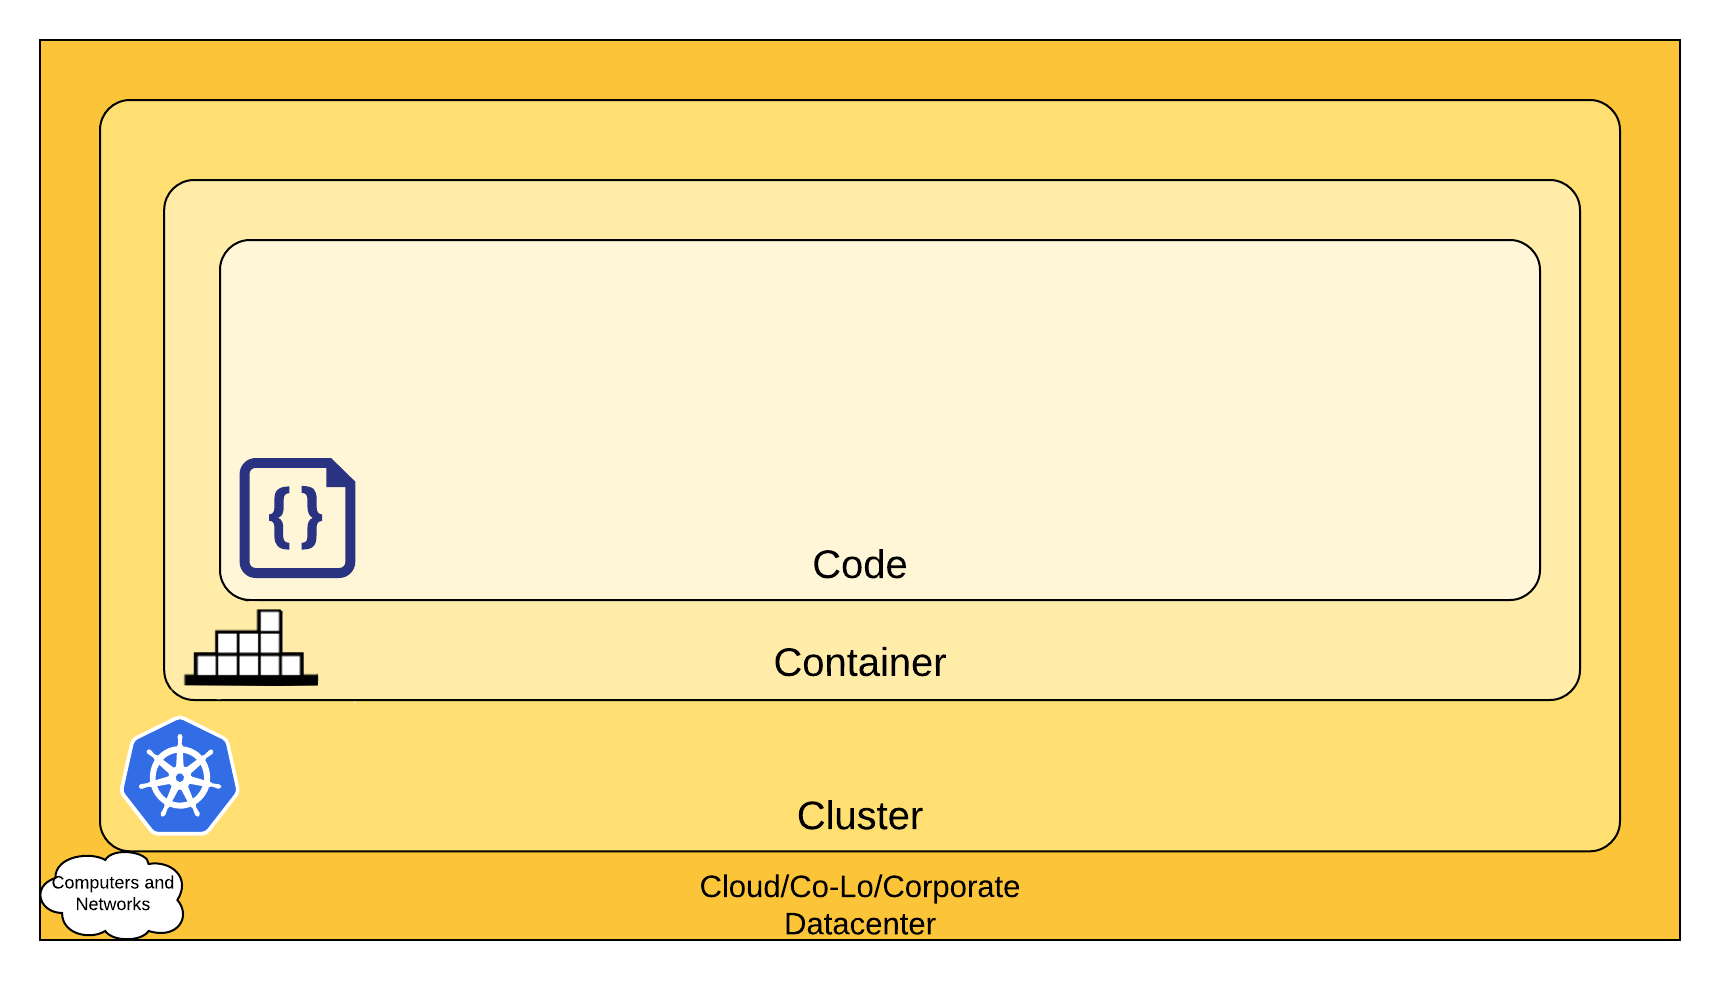
\includegraphics[width=0.75\textwidth]{images/cloud-security.png}
        \caption{Four layers of the cloud infrastructure.}
		\label{img:cloud-security}
	\end{center}
\end{figure}

Each layer is built upon the previous one and its security depends on the security of the outer layers. It is, therefore, important to maintain high security standarts on base levels (cloud, cluster, container).

\begin{enumerate}

\item \textbf{Cloud} \\
Each cloud provider has its own security policies and guidelines. There are, however, some general infrastructure-level security best advice described by in the Tab~\ref{tab:cloud-security-recommendations}.

\begin{table}[H]
    \begin{center}
        \begin{tabular}{ | >{\raggedright\arraybackslash}p{.20\textwidth} 
                         | >{\raggedright\arraybackslash}p{.75\textwidth} | } 
         \hline
         \textbf{Area of Concern for Kubernetes Infrastructure} & \textbf{Recommendation} \\ 
         \hline
         Network access to API Server (Control plane) & All access to the Kubernetes control plane is not allowed publicly on the internet and is controlled by network access control lists restricted to the set of IP addresses needed to administer the cluster. \\ 
         \hline
         Network access to Nodes (nodes)  & Nodes should be configured to only accept connections (via network access control lists) from the control plane on the specified ports, and accept connections for services in Kubernetes of type NodePort and LoadBalancer. If possible, these nodes should not be exposed on the public internet entirely. \\ 
         \hline
         Kubernetes access to cloud provider API & Each cloud provider needs to grant a different set of permissions to the Kubernetes control plane and nodes. It is best to provide the cluster with cloud provider access that follows the principle of least privilege for the resources it needs to administer. \\
         \hline
         Access to etcd & Access to etcd (the datastore of Kubernetes) should be limited to the control plane only. Depending on your configuration, you should attempt to use etcd over TLS. \\
         \hline
         etcd Encryption & Wherever possible it's a good practice to encrypt all storage at rest, and since etcd holds the state of the entire cluster (including Secrets) its disk should especially be encrypted at rest. \\
         \hline
        \end{tabular}
    \end{center}
    \caption{Security recommendations for the cloud layer.}
    \label{tab:cloud-security-recommendations}
\end{table}

\item \textbf{Cluster} \\
There are two cluster security concerns that could be addressed: securing the configurable cluster components and securing the applications running in the cluster.

There are a few things to consider regarding the application security:
\begin{itemize}
\item RBAC Authorization (Access to the Kubernetes API)
\item Authentication	
\item Application secrets management (and encrypting them in etcd at rest)
\item Ensuring that pods meet defined Pod Security Standards
\item Quality of Service (and Cluster resource management)
\item Network Policies
\item TLS for Kubernetes Ingress
\end{itemize}

\item \textbf{Container} \\
Securing containers is a vast topic, which deserves its own chapter. There are, nevertheless, a few general recommendation provided by the Kubernetes, which you can find in the Tab~\ref{tab:container-security-recommendations}.

\begin{table}[H]
    \begin{center}
        \begin{tabular}{ | >{\raggedright\arraybackslash}p{.30\textwidth} 
                         | >{\raggedright\arraybackslash}p{.65\textwidth} | } 
        \hline
        \textbf{Area of Concern for Containers} & \textbf{Recommendation} \\ 
        \hline
        Container Vulnerability Scanning and OS Dependency Security & As part of an image build step, you should scan your containers for known vulnerabilities. \\ 
        \hline
        Image Signing and Enforcement & Sign container images to maintain a system of trust for the content of your containers. \\ 
        \hline
        Disallow privileged users & When constructing containers, create users inside of the containers that have the least level of operating system privilege necessary in order to carry out the goal of the container. \\
        \hline
        \end{tabular}
    \end{center}
    \caption{Security recommendations for the Container layer.}
    \label{tab:container-security-recommendations}
\end{table}

\item \textbf{Code} \\
When it comes to code, the developers have the most flexibility to design secure applications. There are a lot of issues to address, which may vary significantly from application to application depending on its purpose, architecture and framework base. Kubernetes documentation gives a handful of recommendations regarding this topic, which are displayed below in the Tab~\ref{tab:code-security-recommendations}.

\begin{table}[H]
    \begin{center}
        \begin{tabular}{ | >{\raggedright\arraybackslash}p{.20\textwidth} 
                         | >{\raggedright\arraybackslash}p{.75\textwidth} | } 
        \hline
        \textbf{Area of Concern for Code} & \textbf{Recommendation} \\ 
        \hline
        Access over TLS only & If your code needs to communicate by TCP, perform a TLS handshake with the client ahead of time. With the exception of a few cases, encrypt everything in transit. Going one step further, it's a good idea to encrypt network traffic between services. This can be done through a process known as mutual TLS authentication or mTLS which performs a two sided verification of communication between two certificate holding services. \\ 
        \hline
        Limiting port ranges of communication & This recommendation may be a bit self-explanatory, but wherever possible you should only expose the ports on your service that are absolutely essential for communication or metric gathering. \\ 
        \hline
        3rd Party Dependency Security & It is a good practice to regularly scan your application's third party libraries for known security vulnerabilities. Each programming language has a tool for performing this check automatically. \\
        \hline
        Static Code Analysis & Most languages provide a way for a snippet of code to be analyzed for any potentially unsafe coding practices. Whenever possible you should perform checks using automated tooling that can scan codebases for common security errors. \\
        \hline
        Dynamic probing attacks & There are a few automated tools that you can run against your service to try some of the well known service attacks. These include SQL injection, CSRF, and XSS. One of the most popular dynamic analysis tools is the OWASP Zed Attack proxy tool. \\
        \hline
        \end{tabular}
    \end{center}
    \caption{Security recommendations for the Code layer.}
    \label{tab:code-security-recommendations}
\end{table}

\end{enumerate}


\subsection{CIS Kubernetes Benchmark}
\label{sss:cis-kubernetes-benchmark}

CIS publishes a variety of documents for an array of different platforms and infrastructure components. Benchmarks are available for 10 cloud providers, 26 operating systems, 19 kinds of system software, as well as for mobile devices, network devices and desktop software. Benchmarks for the cloud services, for instance, include such cloud providers as Alibaba, Amazon, Google, IBM, Microsoft, Oracle and a few others. For Kubernetes platform, specifically, GKE, AKS, EKS and general Kubernetes benchmarks are available for non-commercial use. 

CIS Benchmark is a PDF file, which contains a list of checks (both manual and automated), that can be performed to ensure the most secure environment. CIS Benchmark file for Kubernetes has 5 categories of security recommendations:
\begin{enumerate}[noitemsep]
    \item Control Plane Components
    \item etcd
    \item Control Plane Configuration
    \item Worker Nodes
    \item Policies
\end{enumerate}

There are multiple subcategories for the most of the categories as well. Each recommendation includes the general information about the check, such as title, description and assessment status. Audit procedure describes the steps necessary to determine if the target system is compliant with the recommendation. Additionaly, every recommendation is supplied with the rationale statement, which gives a ``Detailed reasoning for the recommendation to provide the user a clear and concise understanding on the importance of the recommendation.'' Finally, remediation procedure provides instructions for bringing the the target system into compliance with the recommendation.

CIS Benchmark document \cite{cis-kubernetes-benchmark} states that ```All CIS Benchmarks (Benchmarks) focus on technical configuration settings used to maintain and/or increase the security of the addressed technology, and they should be used in conjunction with other essential cyber hygiene tasks ... In the end, the Benchmarks are designed to be a key component of a comprehensive cybersecurity program.''' This means that even though benchmarks cover many aspects of Kubernetes security, authors recommend to use in combination with other defensinve and monitoring tools.

\subsection{NSA Framework}

The NSA Kubernetes Hardening Guide is a security framework jointly published by the U.S. National Security Agency and CISA. It provides actionable recommendations to secure Kubernetes clusters against real-world threats. As stated in the document itself \cite{nsa-kubernetes-hardening-guide}, it ``describes the security challenges associated with setting up and securing a Kubernetes cluster. It includes strategies for system administrators and developers of National Security Systems, helping them avoid common misconfigurations and implement recommended hardening measures and mitigations when deploying Kubernetes''. First released in August 2021, it was last updated in August 2022, but is still used worldwide as the most of the described concepts are still applicable to the newest Kubernetes versions.

This guide is a well-structured document 66 pages long. It is written as a text guide and divided into multiple sections. The sections are Kubernetes Pod Security, Network Separation and Hardening, Authentication and Authorization, Audit Logging and Threat Detection, Upgrading and Application Security Practices. Each section describes the best security practices for a particular domain. For instance, the document proposes a hardened container build workflow, where each image must pass three security services (image signature verification, image scanner, configuration validation) before being deployed into the cluster. Figure~\ref{img:hardened-container-build-workflow} displays a schematic overview of the workflow. Interstingly, the document references and is partially based on MITRE ATT\&CK Framework.

\begin{figure}[!hbt]
	\begin{center}
		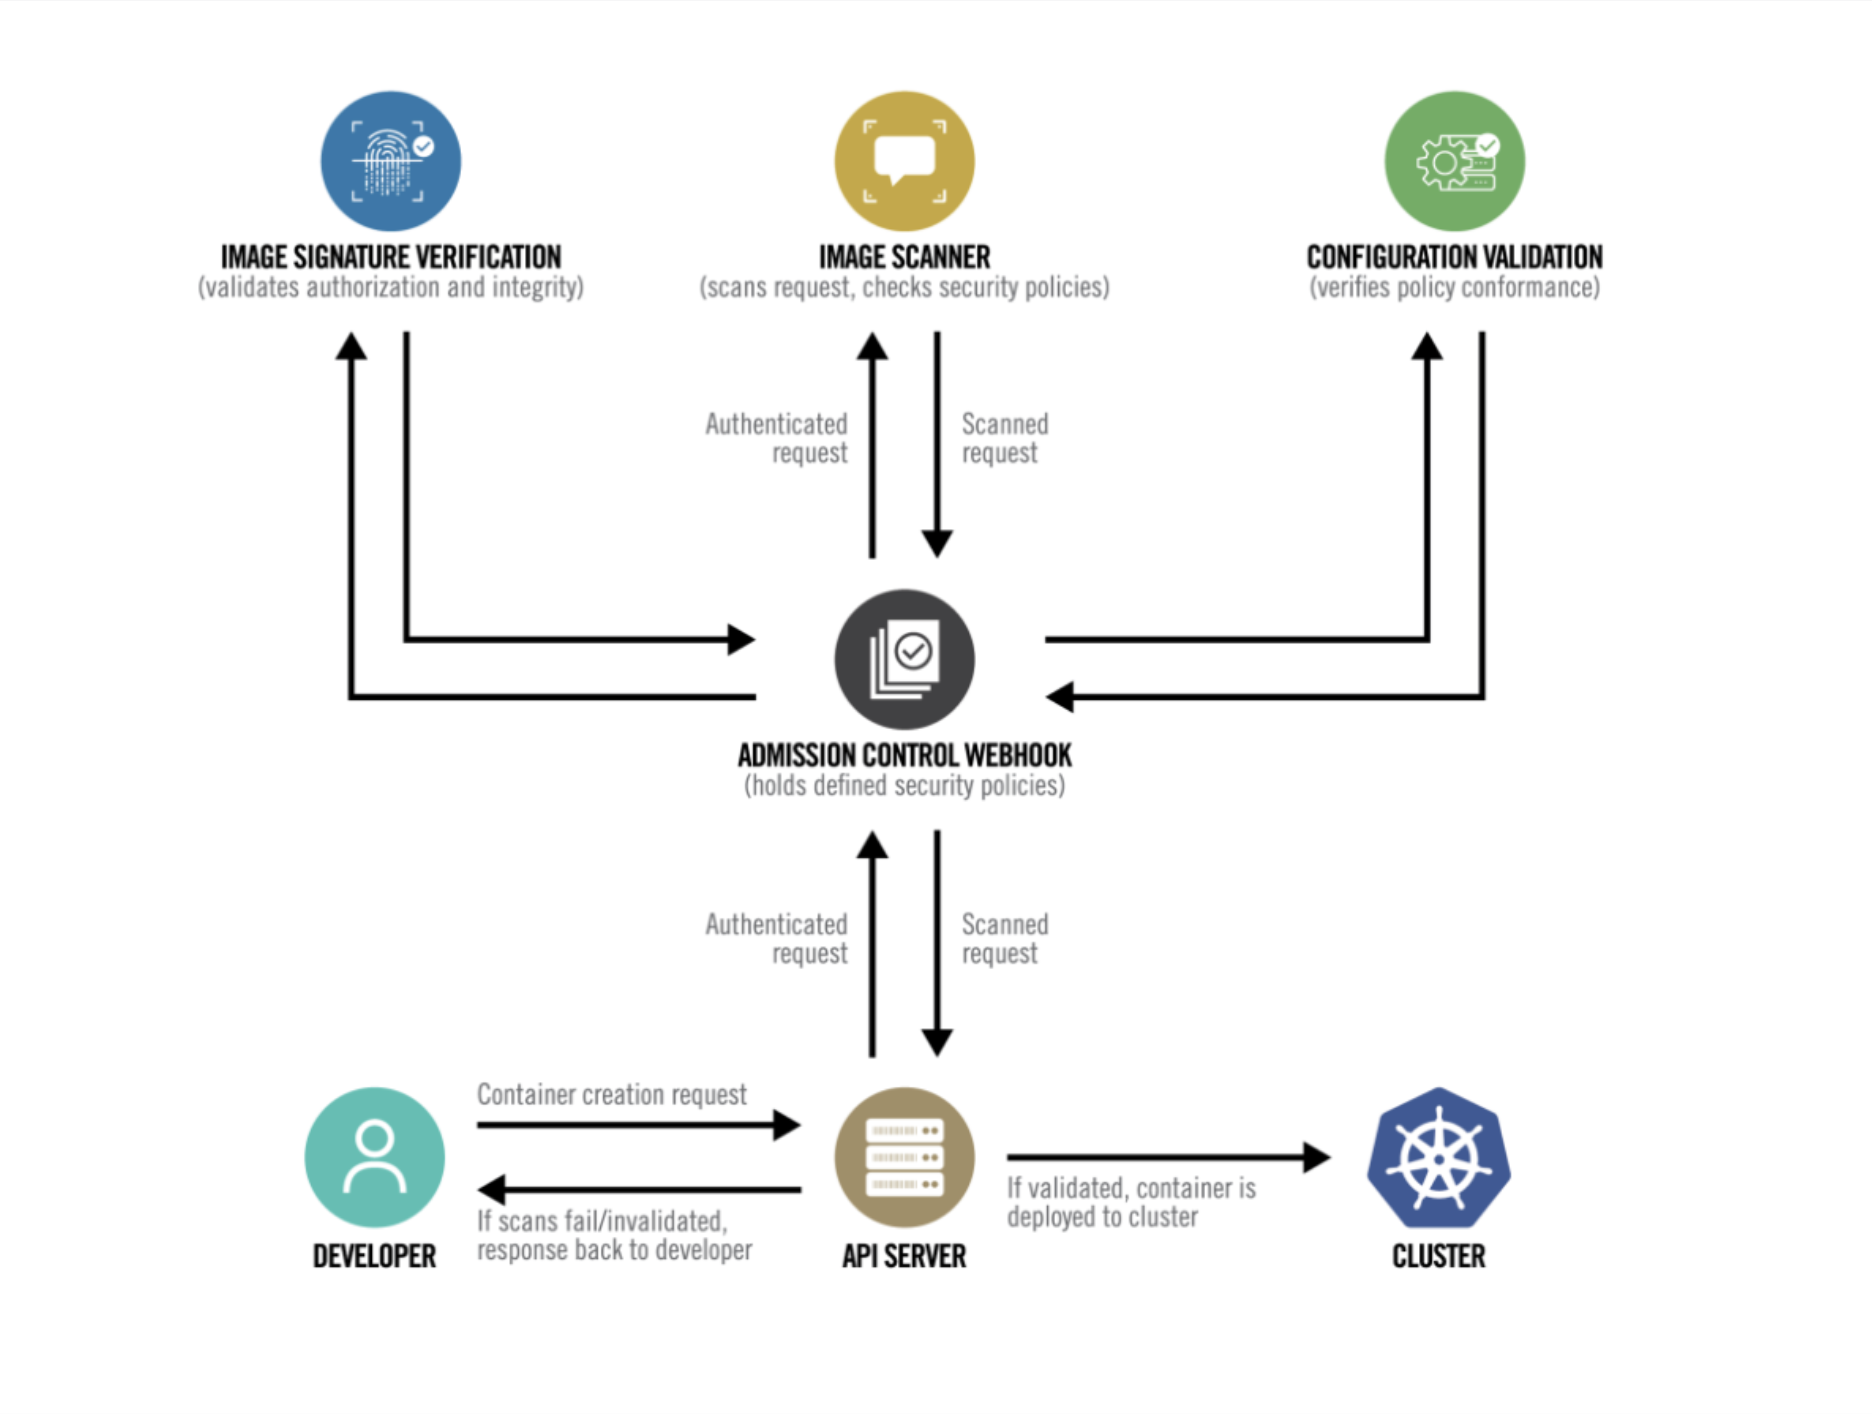
\includegraphics[width=0.9\textwidth]{images/hardened-container-build-workflow.png}
        \caption{A hardened container build worflow.}
		\label{img:hardened-container-build-workflow}
	\end{center}
\end{figure}

\subsection{MITRE ATT\&CK Framework}

The MITRE ATT\&CK Framework (Adversarial Tactics, Techniques, and Common Knowledge) is a comprehensive knowledge base of cyber adversary behavior. It categorizes the tactics and techniques that attackers use across various stages of an intrusion, helping the security specialists to understand, detect, and mitigate real-world threats. Tactics describe the rationale and goals of the attacker, among the most common tactics are Initial Access, Execution, Discovery and Impact. Techniques describe the methods used by the attackers to achieve a tactic. It can be any action from Phishing to Exploitation for Privilege Escalation. Techniques are further granulated into sub-techniques. Finally, Mitigations provide recommendations and controls for each technique while Detection describes the patterns, which can be used to identify technique usage via logs, events and telemetry.

Inside the Kubernetes context, MITRE ATT\&CK Framework publishes techniques for the containerized environments domain. They focus on Kubernetes control plane, worker nodes, pods, and related infrastructure and map known attack behaviors to Kubernetes-specific contexts. For instance, the Initial Access tactic is mapped to the such subtechniques as Compromised Kubeconfig, Exposed Dashboard/API, Impact tactic makes use of Data Destruction (like deleting pods or nodes), Denial of Service and Resource Hijacking techniques. Figure~\ref{img:mitre-attack-matrix} displays the MITRE ATT\&CK matrix for the Container platform.

\begin{figure}[!hbt]
	\begin{center}
		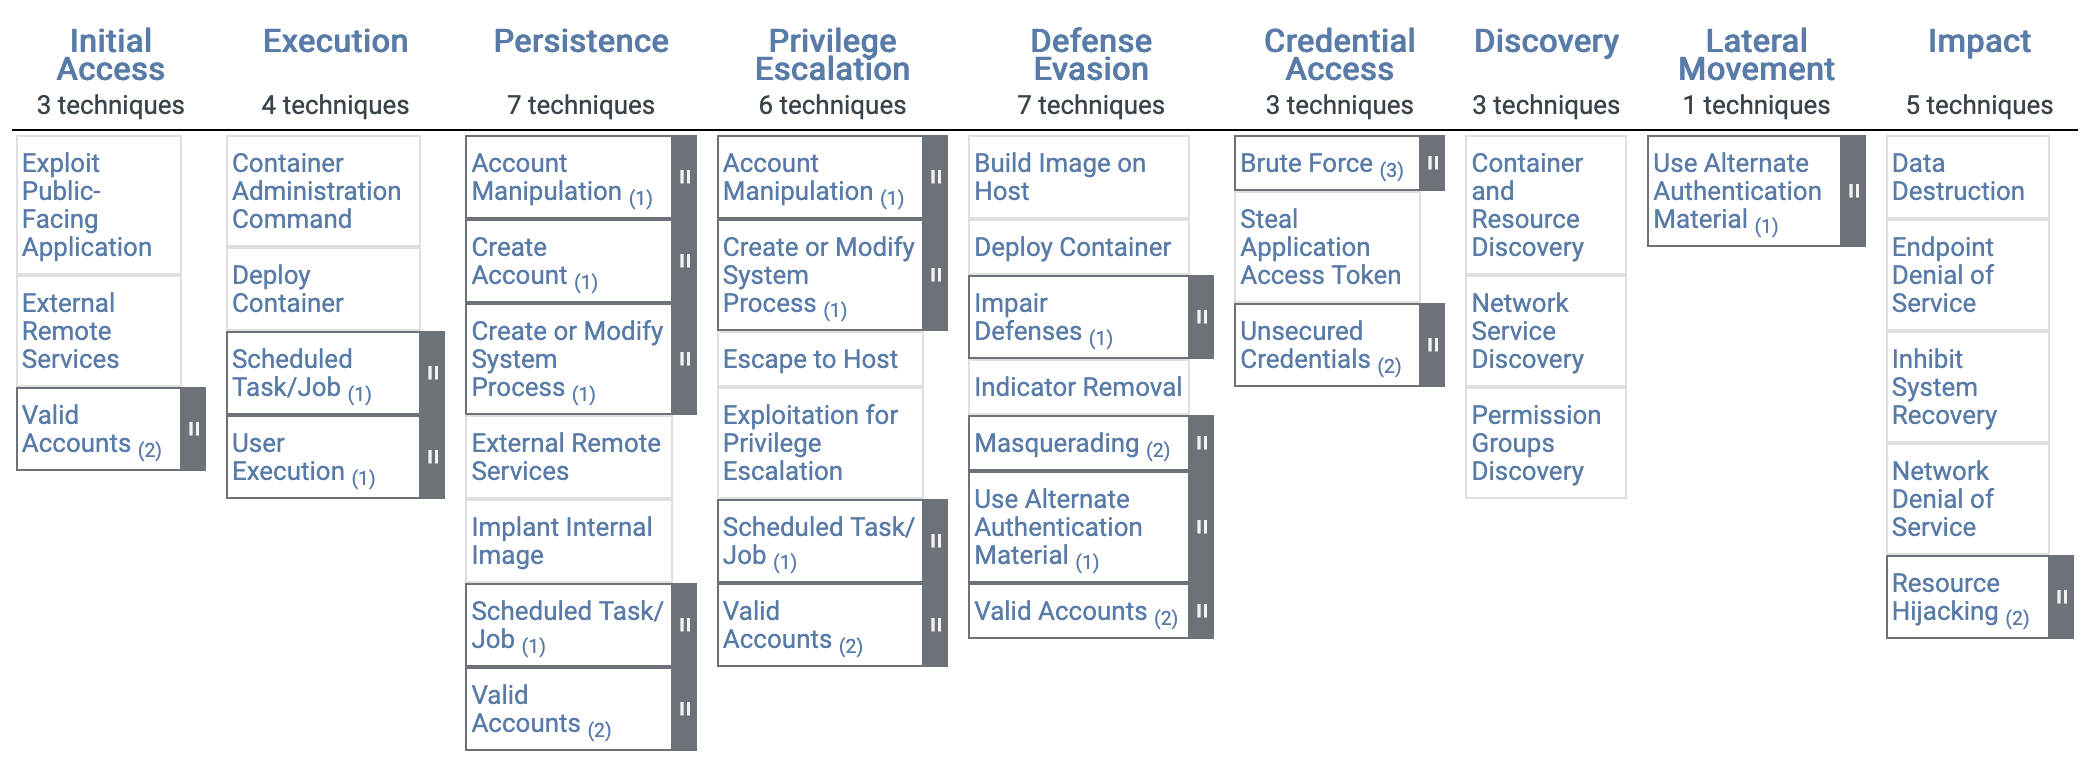
\includegraphics[width=\textwidth]{images/mitre-attack-matrix.png}
        \caption{MITRE ATT\&CK matrix for the Container platform.}
		\label{img:mitre-attack-matrix}
	\end{center}
\end{figure}